In this chapter, we present all experimental results and their analysis.
Section~\ref{section:main_results} shows the main results of the tagging technique and different maximal phrase lengths experiments on different domains. In Section~\ref{section:anlaysis}, to provide further explanations from various perspectives on the findings we perform several analyses. We conduct the additional experiments and report their results in Section~\ref{section:additional_experiments}. 
%of a mix of out-domain sentences and in-domain phrases and minimum lengths of phrases.
%We also believe that manual analysis with translation examples can help a better understanding of the results, therefore, we show output samples that are worth a closer look.

\section{Main Results} \label{section:main_results}
%%%%%%%%% Short description of evaluation %%%%%%%%%%%
We evaluate the quality of NMT models by BLEU (Section~\ref{section:evaluation_metrics}) and compute with \textsc{SacreBLEU} \parencite{post-2018-call}. The phrase-adapted models are compared to the non-adapted baseline model~\parencite{ng-etal-2019-facebook}, and to fine-tuning on the original (non fragmented) dataset. 
This demonstrates the lower and upper bounds of the translation quality improvement by domain adaptation, and objectively evaluates our proposed method. 
%\textit{Baseline} is the pre-trained Fairseq WMT19 news model and \textit{Original data} is fine-tuned NMT models on full sentences of in-domain datasets. 

%%%%%%%%%   MAIN RESULT  %%%%%%%%%%%%%%%
Main results are reported in Table~\ref{tab:main_results}. In all domains, the NMT models fine-tuned on phrases outperform the BLEU scores of the baseline model. 
The effect of maximum phrase length and tagging technique on the translation quality of the phrase-adapted models yields varying results across domains. For EMEA and GNOME domains, the BLUE scores of fine-tuning on phrases nearly reached the scores of fine-tuning on complete sentences. On the other hand, fine-tuning on phrases of the JRC domain achieves a relatively small improvement compared to other domains with a score of up to +1.4 BLEU. 
%consistent  without using any in-domain parallel sentences, improving up to 14 BLEU over unadapted models, and up to 2 BLEU over strong back-translation baselines.

\begin{table}[hb!]
\centering
\begin{tabular}{c|c|ccccccc}
\Xhline{3\arrayrulewidth}
\multirow{4}{*}{} &
  \multirow{4}{*}{{\begin{tabular}[c]{@{}c@{}} \textbf{Baseline} \\ \textit{(No fine-tune)}\end{tabular}}} &
  \multicolumn{7}{c}{\textbf{Fine-tuning}} \\ \cline{3-9} 
 &
   &
  \multicolumn{6}{c|}{\textbf{Phrase pairs}} &
  \multirow{3}{*}{{\begin{tabular}[c]{@{}c@{}} \textbf{Original data}\\ \textit{(Sentences)}\end{tabular}}} \\ \cline{3-8}
 &
   &
  \multicolumn{2}{c|}{\textbf{Dictionary}} &
  \multicolumn{2}{c|}{\textbf{Max length 4}} &
  \multicolumn{2}{c|}{\textbf{Max length 7}} &
   \\ \cline{3-8}
 &
   &
  \multicolumn{1}{c|}{\textbf{No Tag}} &
  \multicolumn{1}{c|}{\textbf{Tag}} &
  \multicolumn{1}{c|}{\textbf{No Tag}} &
  \multicolumn{1}{c|}{\textbf{Tag}} &
  \multicolumn{1}{c|}{\textbf{No Tag}} &
  \multicolumn{1}{c|}{\textbf{Tag}} &
   \\ \hline \hline
  \textbf{EMEA} &
  35.5 &
  \multicolumn{1}{c|}{36.4} &
  \multicolumn{1}{c|}{38.0} &
  \multicolumn{1}{c|}{39.1} &
  \multicolumn{1}{c|}{40.5} &
  \multicolumn{1}{c|}{41.5} &
  \multicolumn{1}{c|}{37.2} &
  45.2 \\ 
\textbf{GNOME} &
  29.8 &
  \multicolumn{1}{c|}{29.7} &
  \multicolumn{1}{c|}{33.5} &
  \multicolumn{1}{c|}{36.0} &
  \multicolumn{1}{c|}{37.0} &
  \multicolumn{1}{c|}{35.8} &
  \multicolumn{1}{c|}{36.8} &
  38.9 \\ 
\textbf{JRC} &
  29.0 &
  \multicolumn{1}{c|}{28.8} &
  \multicolumn{1}{c|}{30.4} &
  \multicolumn{1}{c|}{29.4} &
  \multicolumn{1}{c|}{30.0} &
  \multicolumn{1}{c|}{29.2} &
  \multicolumn{1}{c|}{29.7} &
  54.7 \\ \Xhline{3\arrayrulewidth}
\end{tabular}
\caption{Main results : BLEU scores of German-English NMT in three different domains: medical (EMEA), software (GNOME), and legal (JRC). The baseline is the pre-trained Fairseq WMT19 news system \parencite{ng-etal-2019-facebook} based on Transformer \parencite{vaswani2017attention} and ranked first in the WMT19 competition. For fine-tuning on phrase pairs, multiple maximum phrase lengths (1 (dictionary), 4 and 7) are used with and without tags.}
\label{tab:main_results}
\end{table}

Besides BLEU, we report the average lengths of the translations from all the NMT models in Figure~\ref{fig:average_length_results}: the baseline, fine-tuning on maximum phrase length 4 with and without tags and fine-tuning on the original full sentences. Sentence length is measured by the total amount of space-separated tokens. We compare them with reference sentences to examine brevity issue. As we expected, in general, the non-tagged phrase-adapted models generate shorter translations than the reference and the baseline and the full-sentence adapted models. Adding tags on phrases improves the bias of short sentence.

% \begin{figure}[h!]
% \centering
% \begin{subfigure}{.48\textwidth}
%   \centering
%   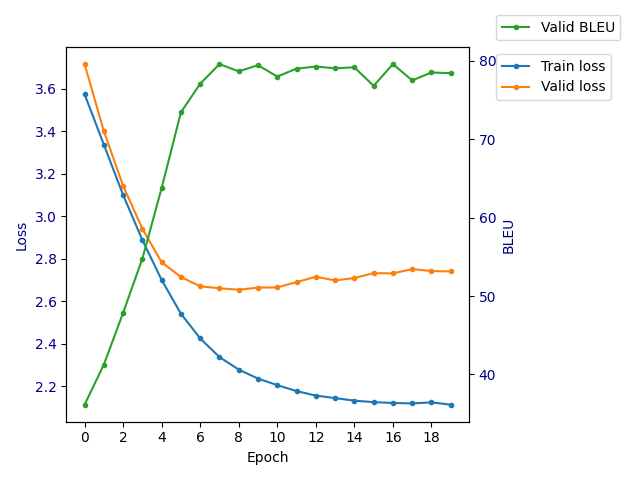
\includegraphics[scale=0.48]{images/EMEA_all.png}
%     \caption{}
%     \label{fig:EMEA_full}
% \end{subfigure}
% \begin{subfigure}{.48\textwidth}
%   \centering
%   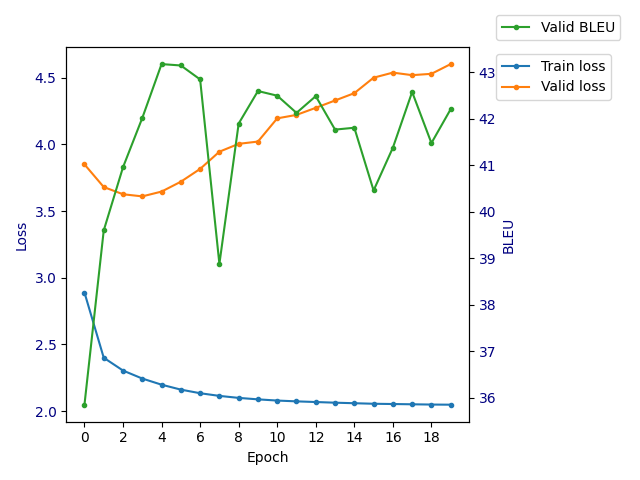
\includegraphics[scale=0.48]{images/EMEA_phrase.png}
%     \caption{}
%     \label{fig:EMEA_phrase}
% \end{subfigure}

% \begin{subfigure}{.48\textwidth}
%   \centering
%   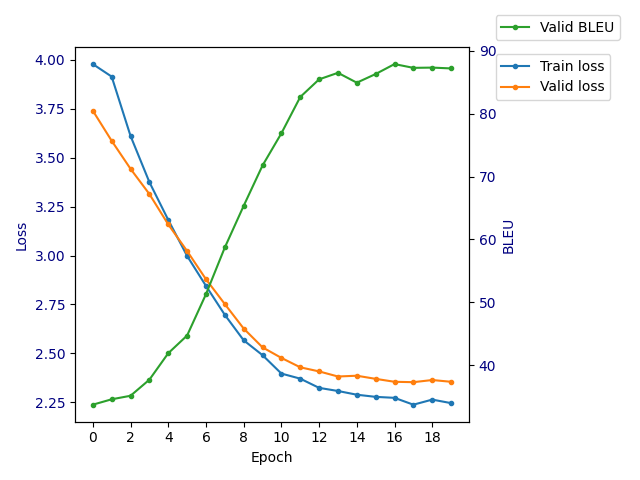
\includegraphics[scale=0.48]{images/GNOME_all.png}
%     \caption{}
%     \label{fig:GNOME_full}
% \end{subfigure}
% \begin{subfigure}{.48\textwidth}
%   \centering
%   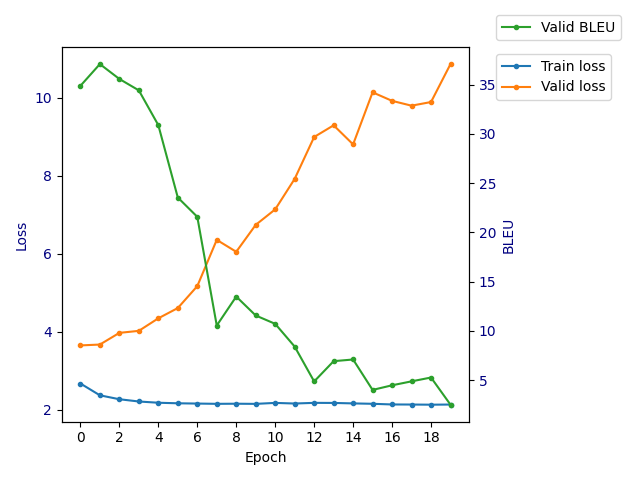
\includegraphics[scale=0.48]{images/GNOME_phrase.png}
%     \caption{}
%     \label{fig:GNOME_phrase}
% \end{subfigure}

% \begin{subfigure}{.48\textwidth}
%   \centering
%   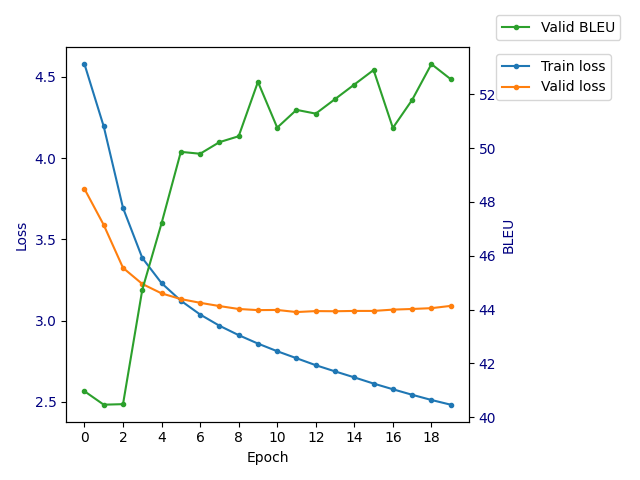
\includegraphics[scale=0.48]{images/JRC_all.png}
%     \caption{}
%     \label{fig:JRC_full}
% \end{subfigure}
% \begin{subfigure}{.48\textwidth}
%   \centering
%   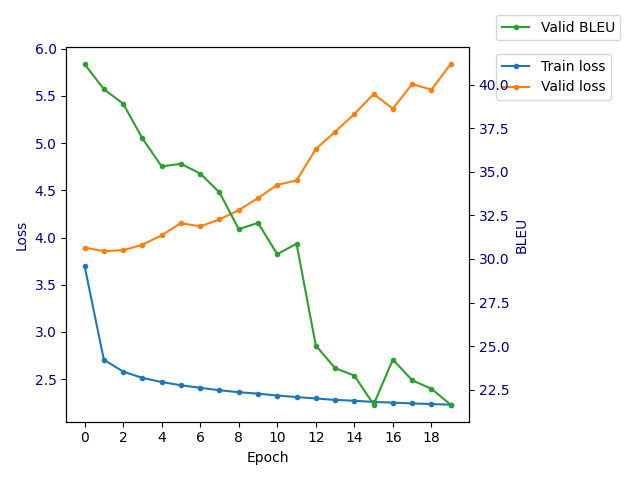
\includegraphics[scale=0.48]{images/JRC_phrase.png}
%     \caption{}
%     \label{fig:JRC_phrase}
% \end{subfigure}
% \caption{}
% \label{fig:fine-tuning-graph}
% \end{figure}

%Main findings - phrase works for fine-tuning 
Our main finding is that phrase pairs can indeed be used to fine-tune a NMT model without any changes to the architecture or the need of specific fine-tuning algorithms. It is relevant for our scenario because even translation companies without significant in-house NMT expertise could easily apply our solution to their workflow. Our approach is also applicable in cases where translation company \textbf{\textit{A}} uses NMT as an outsourced (cloud-based) service, by sending the provider phrase pairs instead of full sentences for model adaptation. In the following, we describe in depth the effects of the tagging technique, phrase length and domains on the main results.

%NMT system is provided by an external (cloud-based) provider and the translation company 
\subsection{Effect of phrase tagging}%%%%%%%%%%%%%%%%%%%%%%%%%%%%%%%

We expected that the tagging technique would help an NMT system differentiate between the phrase and the original dataset and eventually could improve translation quality. In most cases, adding tags to phrases increase the BLEU scores, gaining up to +3.8 BLEU (fine-tuning on the GNOME domain with maximum length 1).
%For most other phrase lengths except dictionaries (i.e. maximum phrase length of 1), even without tagging, domain adaptation using phrases outperform the baseline.
%In the case of the dictionary (i.e. maximum phrase length of 1), except on EMEA, without tagging, it does not have an advantage due to domain adaptation, and when the tagging technique is applied, the score increases significantly more than the scores shown in other lengths.
In addition, tagging technique seems to be more effective, especially for short phrases. When NMT is fine-tuned on dictionaries of in-domain datasets (i.e., maximum phrase length of 1), without tags, the model cannot take advantage of domain adaptation in the GNOME and JRC domains, but with tags, the increase in BLEU score stands out compared to other longer phrase lengths.
%the increase in BLEU score over un-tagged phrases is noticeable compared to other phrase lengths in all domains. 

Figure~\ref{fig:average_length_results} shows that tagging yields to slightly longer system outputs, suggesting the model indeed learned to associate the <PT>, </PT> tag with shorter training samples.
While differences look small, they have a large impact on BLEU because of the Brevity Penalty \parencite{papineni-etal-2002-bleu}.
As a notable exception to this positive trend, BLEU score decreases with tagging on EMEA with maximum length 7. 
%We are currently investigating this result further.
%We expected the tagging system to help the model to differentiate between the phrase dataset and the original dataset, but this did not significantly improve the models performance.

\subsection{Effect of phrase length}\label{section:effect_phrase_length}

We expected that longer phrases to be considerably more useful for fine-tuning NMT models than short ones. This is because longer phrases may have more contextual information, at the expense of less confidentiality protection. 
However, experimental results for three different maximum phrase lengths (1, 4 and 7) show that the increase in phrase length is not proportional to the increase in BLEU.
% When fine-tuning on the dictionary of each domain, only the EMEA domain increased the BLEU score (+1.6), and the other domains decreased the score very finely. 
The NMT models fine-tuned on phrases with a maximum length of 1 have a higher BLEU score (+1.6) than the baseline model only in the EMEA domain and decrease slightly in other domains. Fine-tuning on a maximum length of 4 phrases results in higher BLEU scores than dictionary-adapted models (except for tagged JRC domains). By contrast, increasing the maximum length from 4 to 7 does not have a positive effect on BLEU but actually lowers it in the GNOME and JRC domains. This counter-intuitive result may be due to the fact that increasing the maximum length leads to a much larger number of extracted phrases that are redundant and overlapping. Previous work on lexicon-augmented NMT also reported negative results when fine-tuning on very large numbers of segments \parencite{thompson-etal-2019-hablex}.
%, we plan to experiment with minimum phrase length as a way to reduce the total number of phrase pairs. % without losing translation knowledge.

\subsection{Domain differences}~\label{section:domain_defference}%%%%%%%%%%%%%%%%%%%%

The benefits of fine-tuning on phrases appear to vary strongly across domains: on EMEA we obtain large gains but there is still space for improvement, on GNOME our approach nears the maximum gain achievable with original data fine-tuning, whereas on JRC gains are small and scores remain very far from the ceiling. 
%maximum gain achievable with original data fine-tuning.
%Furthermore, we can see that the difference between domains is significant. For instance, EMEA generally works better with phrases than the other domains. Conversely, 
To explain these results, we inspected our in-domain datasets and specifically looked for peculiarities of the JRC dataset. We find that JRC is rather different in terms of sentence length distribution, with much longer sentences on average. As shown in Figure~\ref{fig:average_length_results}, only fine-tuning on original data leads to reasonably long outputs, whereas baseline and phrase-adapted systems all generate sentences that are, on average, about 10 words shorter then they should be. This suggests that our tagging technique is not sufficient to address the shorter-output bias in a robust way.
% James Kirkpatrick, Razvan Pascanu, Neil Rabinowitz, Joel Veness, Guillaume Desjardins, Andrei A Rusu, Kieran Milan, John Quan, Tiago Ramalho, Ag- nieszka Grabska-Barwinska, et al. 2017. Overcoming catastrophic forgetting in neural networks.
%The baseline model on EMEA outperformed other domains, but for the fine-tuned NMT models on original data, on JRC gained +25.7 BLEU while other models gained around +10 BLEU scores each. 
% For the intervals of the lower and upper bounds of BLEU score in domains, JRC has + 25.7 BLEU 
% This indicates that JRC domain has the biggest room for domain adaptation improvement in BLEU score compared to the other domains.

\begin{figure}[hb!]
    \centering
    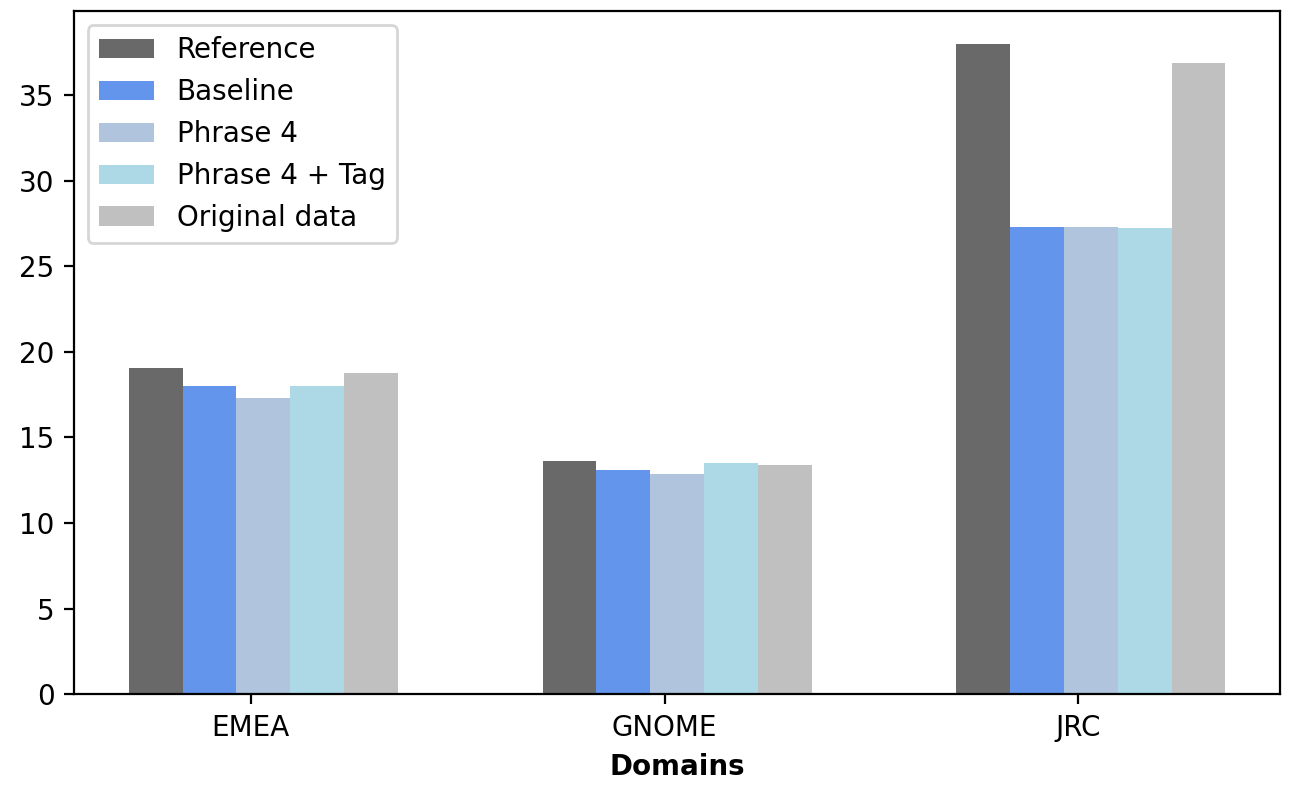
\includegraphics[scale=0.7]{images/average_result.png}
    \caption{Average length (in words) of reference translations and outputs of different NMT systems.}
    \label{fig:average_length_results}
\end{figure}

%\AB{IMPORTANT: cite somewhere papers that train MT on dictionaries/lexicons} \\
%- HABLex :\cite{thompson-etal-2019-hablex} \\
% CAMERA-READY cite this! - Bridging Neural Machine Translation and Bilingual Dictionaries \cite{zhang2016bridging}
%- It is the different between the domain specificity? ; \\

%Generally JRC has way longer and way more unique sentences. Even there are almost no duplicate. Thus, probably JRC dataset could have more information and context than other two domains. Furthermore, the number of extracted phrases from JRC dataset was way more than others( more than 100k phrases). 
%Firstly, I checked up the EMEA and GNOME datasets and their sentences are way shorter than JRC. Furthermore, these both datasets have lots of duplicates( for the training sets, more than 60\% are duplicate sentences..). Even I filtered out duplicate sentences quite a lot  last time, but I couldn’t remove all of them due to working with the separate documents level to keep the information that which sentences from which documents. And also I wasn't sure how much I should filtered out this duplicates. How does normally researchers remove these duplicates? 
%Furthermore, in this case, probably then EMEA, GNOME test sets are easier than JRC test set. So I will change at least for the tests sets for EMEA and GNOME. However, my concern is that it is also might be the specificity of these domain datasets. Then, if I only get the unique sentences for the experiments, maybe it’s a bit too much intervention. I was just wondering how you think about it?
%Also another possible explanation is while extracting the phrases from the datasets, the more frequent/important(?) words will be extracted as more amounts of phrases. In other words, EMEA and GNOME might has more frequently used words as their domain and also their datasets have heavy duplicates. Then the phrases might be more selected words for translation even they lost lot’s of context information. I am not so sure it make sense or not though. Therefore, I’m fine-tuning the model with randomly 50\% selected phrases for the all datasets to check this randomly selecting might work better for our hypothesis.
%Also I think it might be overfitting. I will also plot the losses and check it out as well.

\section{Analysis}\label{section:anlaysis} %%%%%%%%%%%%%
%In this section, we perform an in-depth analysis 
In the previous section, we presented the main experimental results. It clearly indicates that using phrases with tags for fine-tuning NMT models can achieve translation quality improvements. In this section, we analyse the in-domain datasets and all the fine-tuned models (on tagged phrases and full sentences) in more depth to gain some insights from the results.
%It shows that the effectiveness of our method varies significantly across domains, especially in the JRC domain. %Through this analysis, we aim to explain the following questions: Therefore, through this analysis, we aim to gain more insights into our work. %the effectiveness of our presented method.
% \begin{enumerate}
%     \item Why different 
%     \item Why does fine-tuning on JRC have very small improvement compared to others?
% \end{enumerate}
%What does transfer learning improve? i.e. which classes benefit the most from transfer learning?
%Therefore, by investigating the differences between domains, we eventually aim to better explain the effectiveness of the proposed method.
%Therefore, by investigating the differences between domains so that we can eventually better explain the effectiveness of our presented method.

\subsection{Domain analysis}%%%%%%%%%%%%%%%%%%%%%%%%%%%%

% domain has their own specificity and some features may affect to our results. We inspect 1) different lengths 2) vocabulary 3) similarity between training / test sets 4) fine-tuning process : overfitting 5) Qualitative analysis:translation examples
%Every domain probably has its own specificity. In order to gain more insight into our results, we inspected the characteristic of each domain dataset.
%Every domain has its own characteristics, and an NMT model learns it through domain adaptation. We assume that these features will still be present in the fragmented in-domain data set, and we think that the impact of the proposed method will vary from domain to domain. 
In this thesis work, we applied our proposed method to three different technical domains. Every domain has its characteristics, and an NMT model learns them while fine-tuning the target domain sentences. However, our approach is using fragmented sentences --- phrase pairs --- instead of whole sentences for fine-tuning. 
According to the main results, phrase-adapted NMT models were unable to reach the BLEU scores of the fine-tuned NMT models on full sentences, and how close these models reached their upper bound differed significantly across domains. We explore how domain specificity affects domain adaptation in phrases through several analyses.
%When the domain-adapted model with full sentences is considered as the maximum upper bound that can be reached with domain adaptation, according to the main results, the difference in the phrase-adapted models showed a large difference depending on the domain. According to the main results, phrase-adapted models cannot reach as much as the BLEU scores of the model fine-tuned on full sentences and how close the phrase-adapted models came to this upper bound differed significantly across domains.

\subsubsection{Sentence length differences in domains}

As we mentioned in Section~\ref{section:domain_defference}, we discovered that the average sentence length is significantly different across every domain. To take a closer look, we report the distribution of German sentence lengths for all domains in Figure~\ref{fig:Lengthofsentences}. %, clearly showing that the each domain has different distribution of sentence lengths. 
It is clear that the JRC domain data consists of longer sentences than other domains, while most sentences of the GNOME domain are less than 20 words. In the main results, the JRC domain has the biggest room for potential BLEU gain of domain adaptation but using phrases of JRC for fine-tuning improved only +1.4 BLEU. 
On the other hand, fine-tuning on phrases of the GNOME domain reached close to the maximum potential gain of the BLEU score. 
%When we train NMT models on short phrases, it may give good translations for short sentences but may not for long sentences. 
We may explain this with the following assumption: Training NMT models on short phrases may give good translations for short sentences and less good for long sentences. Thus, when evaluating phrase-adapted models, domains with long sentences may have a disadvantage in scoring BLEU compared to other domains, as they may translate less good for long test sentences.  

% as your model is trained on long sentences, it gives good translations with long sentences. So simply the solution to get good translations with short sentences is to add shorter sentences (maybe split from longer ones) to your training dataset. When I did that, I got better translations for shorter sentences, but when I exaggerated in adding too many short phrases (I extracted several possibilities), some translations included unnecessary words and the overall BLEU was lower. So to conclude, you need short sentences/phrases in your training dataset; however, do not exaggerate by adding too many short sentences that are much more than the original number of long sentences, especially if your domain usually has more long sentences than short ones. It is a trade off; so you have to identify your priorities.

\begin{figure}[hb!]
\centering
\begin{subfigure}{.32\textwidth}
  \centering
  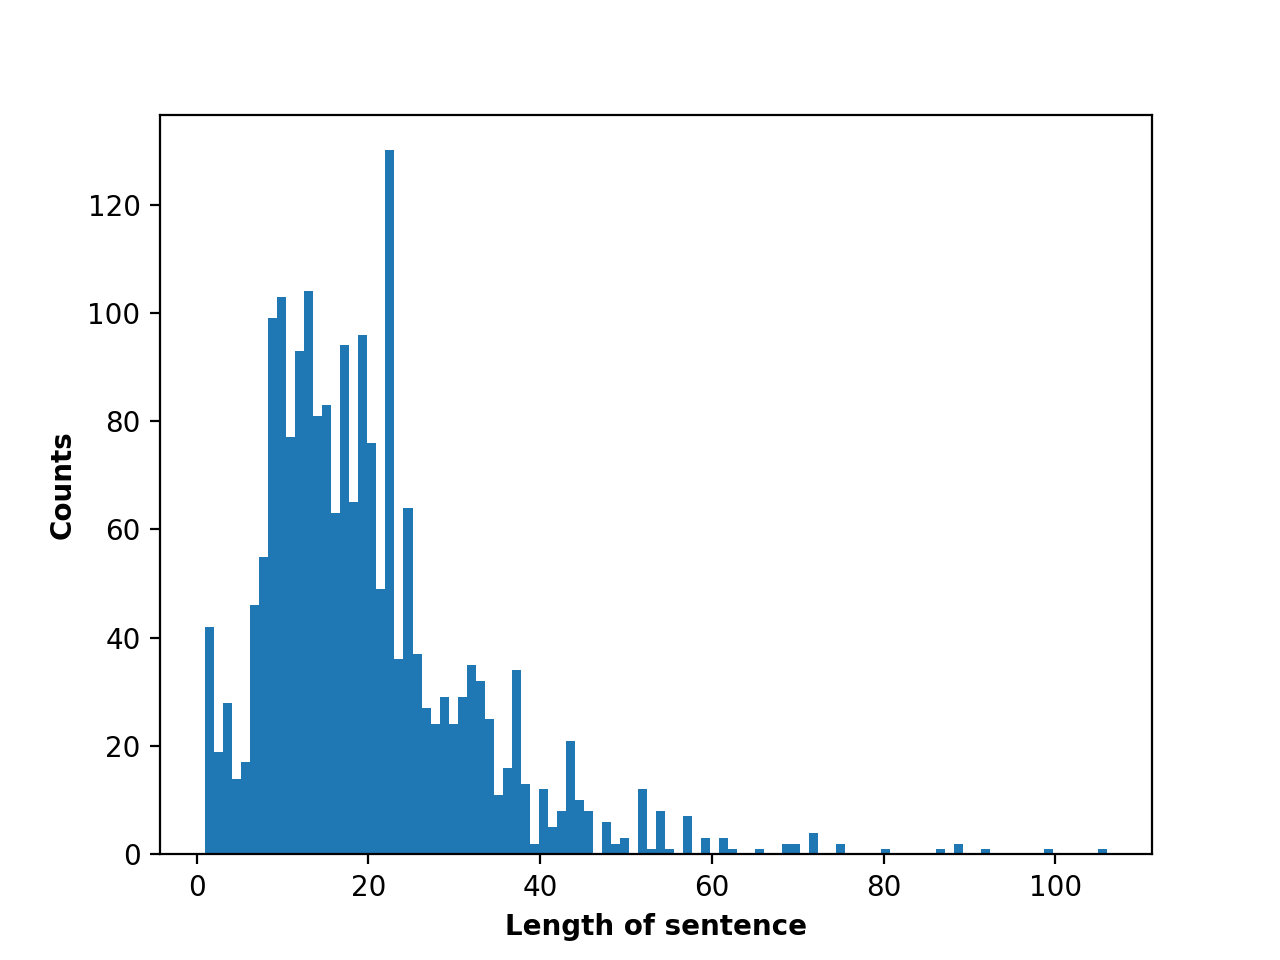
\includegraphics[width=1\linewidth]{images/EMEA_length.png}
  \caption{EMEA test set}
  \label{fig:sub1}
\end{subfigure}
\begin{subfigure}{.32\textwidth}
  \centering
  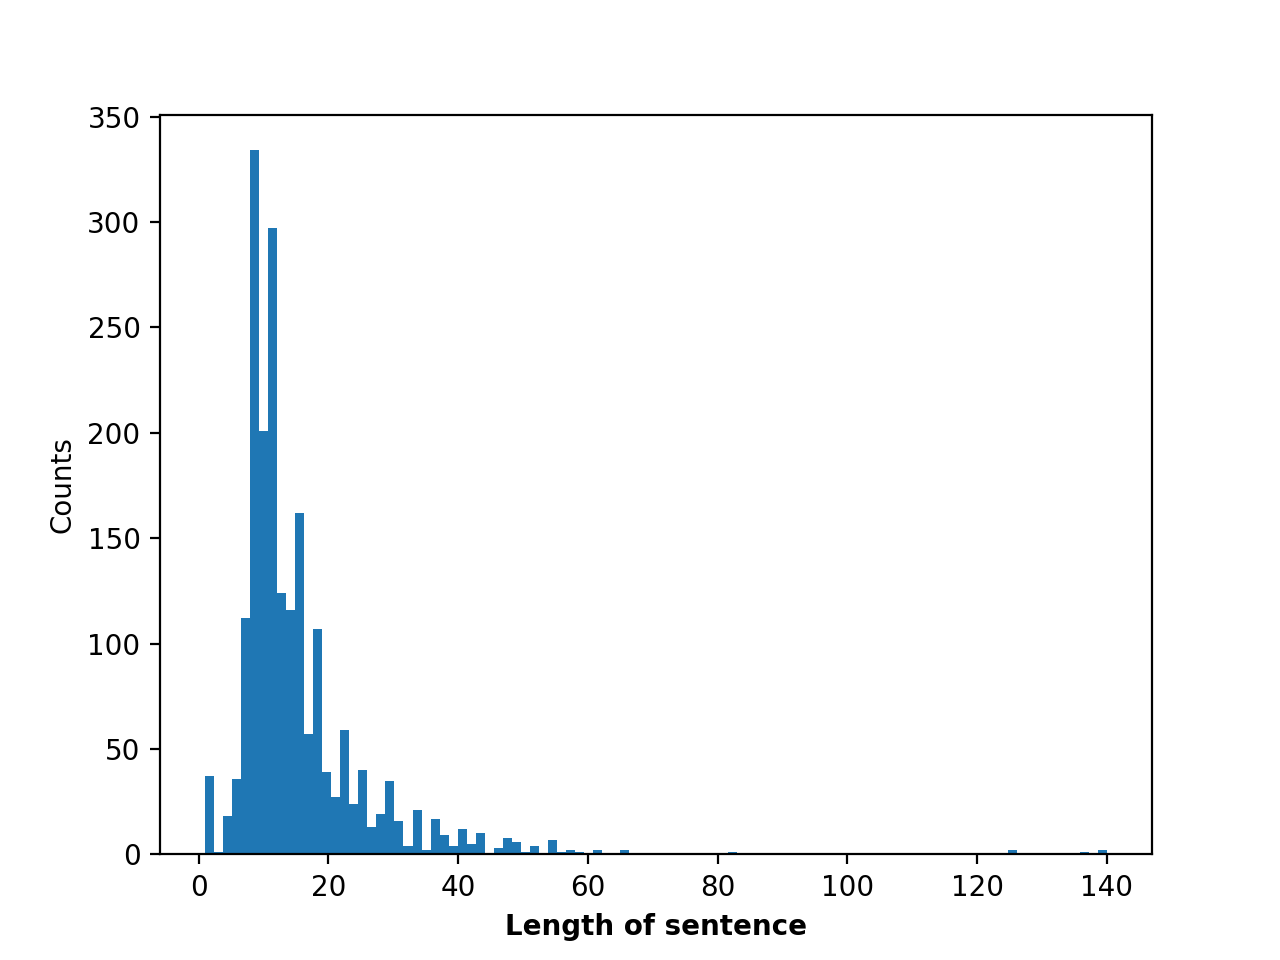
\includegraphics[width=1\linewidth]{images/GNOME_length.png}
  \caption{GNOME test set}
  \label{fig:sub1}
\end{subfigure}
\begin{subfigure}{.32\textwidth}
  \centering
  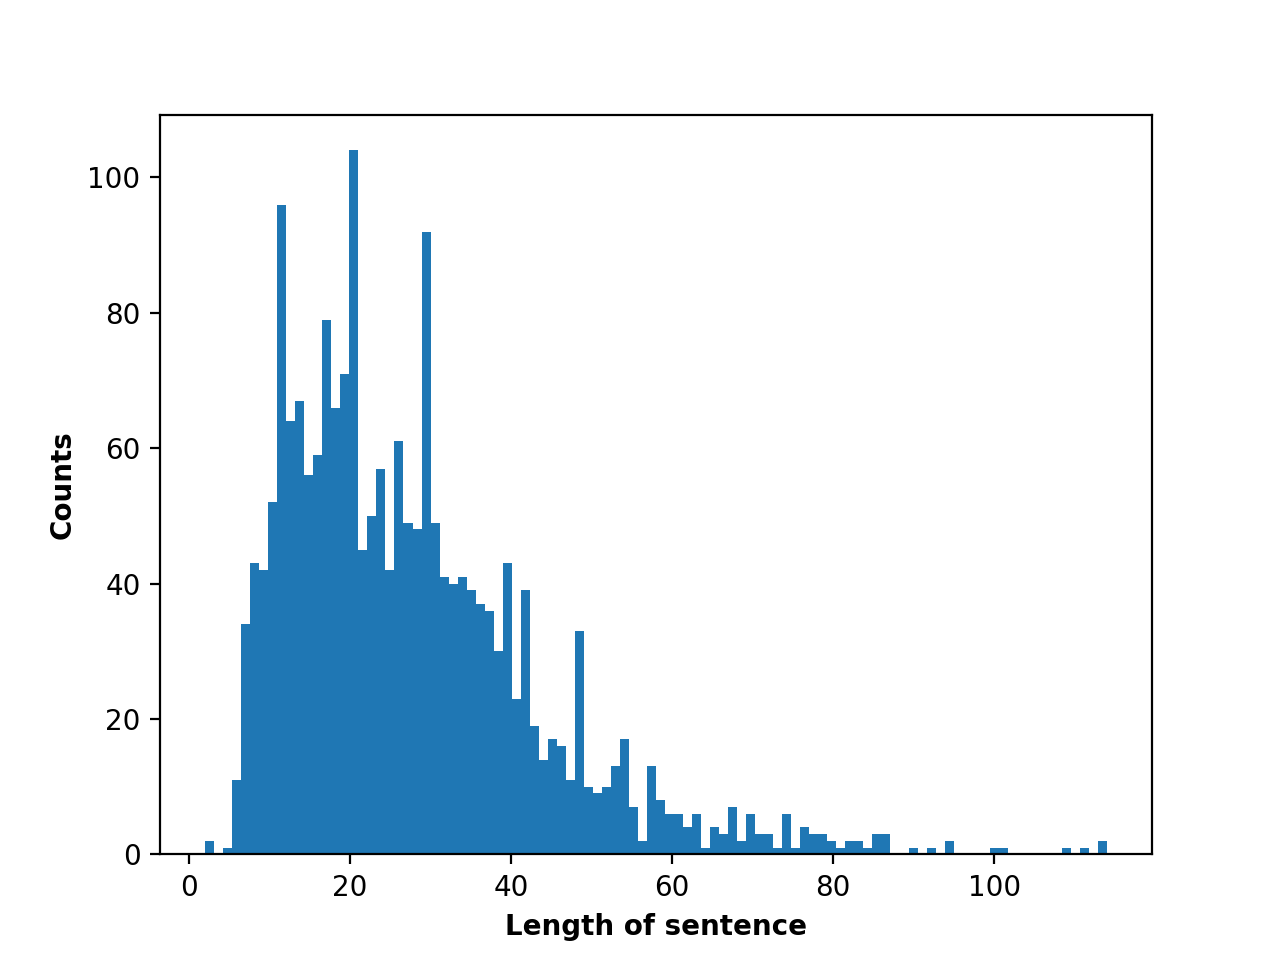
\includegraphics[width=1\linewidth]{images/JRC_length.png}
  \caption{JRC test set}
  \label{fig:sub2}
\end{subfigure}
\caption{German sentence length distributions for each domain's test set. }
\label{fig:Lengthofsentences}
\end{figure}

%Specifically, through this, we attempt to answer the following questions: 1) Is it really that models fine-tuned on phrase outperform short sentence translations than models fine-tuned with long sentences? 2) When comparing the performance between domains, do domains with relatively short sentences perform better for short sentences and poorer for long sentences than domains with long sentences?
To verify this assumption, we investigate whether the phrase-adapted models in each domain show translation quality differences for different length sentences. 
We re-evaluate all NMT models with test sets of different sentence lengths: baseline model, the models fine-tuned on tagged phrases in maximum length 4 and the models fine-tuned on the original full sentences. 
We split the test set for each domain into three different sentence lengths: short ($1\sim9$ words), middle ($10\sim19$ words) and long($20\sim$ words). The numbers of short, medium and long sentences of the each domain's test set are described in Table~\ref{tab:lenght_of_sentences}. 

\begin{table}[h!]
\centering
\begin{tabular}{cclclcl}
\Xhline{3\arrayrulewidth}
\multirow{2}{*}{} & \multicolumn{6}{c}{\textbf{Sentence length of testset}}                                                                 \\ \cline{2-7} 
                  & \multicolumn{2}{c}{\textbf{Short} ($1\sim9)$} & \multicolumn{2}{c}{\textbf{Middle} ($10\sim19)$} & \multicolumn{2}{c}{\textbf{Long} ($20\sim)$} \\ \hline
\textbf{EMEA}     & \multicolumn{2}{c}{320}            & \multicolumn{2}{c}{859}             & \multicolumn{2}{c}{822}           \\ \hline
\textbf{GNOME}    & \multicolumn{2}{c}{538}            & \multicolumn{2}{c}{1064}            & \multicolumn{2}{c}{399}           \\ \hline
\textbf{JRC}      & \multicolumn{2}{c}{133}            & \multicolumn{2}{c}{610}             & \multicolumn{2}{c}{1258}          \\ \Xhline{3\arrayrulewidth}
\end{tabular}
\caption{Number of sentences in the test set divided by short, medium and long sentence length.}
\label{tab:lenght_of_sentences}
\end{table}

\begin{table}[]
\centering
\begin{tabular}{ccccc}
\Xhline{3\arrayrulewidth}
\multirow{2}{*}{} &
  \multirow{3}{*}{\textbf{Test set}} &
  \multirow{3}{*}{\begin{tabular}[c]{@{}c@{}}\textbf{Baseline}\\ (No fine-tuning)\end{tabular}} &
  \multicolumn{2}{c}{\textbf{Fine-Tuning}} \\ \cmidrule(lr){4-5} 
                                &        &       & \begin{tabular}[c]{@{}c@{}} \textbf{Tagged phrases}\\ (Max length 4)\end{tabular} & \multicolumn{1}{l}{\textbf{Original data}} \\ \cmidrule(lr){2-5}
\multirow{4}{*}{\textbf{EMEA}}  & Short  & 16.8 & 23.0 & 33.8 \\ %\cline{2-5} 
                                & Middle & 35.8 & 43.2 & 48.2 \\ %\cline{2-5} 
                                & Long   & 37.8 & 41.1 & 45.3 \\ \cline{2-5}
                                
                                & All    & 35.5 & 40.5 & 45.2 \\ \hline 
\multirow{4}{*}{\textbf{GNOME}} & Short  & 21.3 & 28.3 & 35.5 \\ %\cline{2-5} 
                                & Middel & 26.5 & 34.9 & 37.6 \\ %\cline{2-5} 
                                & Long   & 36.8 & 41.8 & 41.8 \\ \cline{2-5} 
                                & All    & 29.8 & 37.0 & 38.9 \\ \hline 
\multirow{4}{*}{\textbf{JRC}}   & Short  & 32.6 & 37.8 & 48.8 \\ %\cline{2-5} 
                                & Middle & 31.4 & 33.4 & 52.4 \\ %\cline{2-5} 
                                & Long   & 28.5 & 29.0 & 55.3 \\ \cline{2-5}
                                & All    & 29.0 & 30.0 & 54.7 \\ \Xhline{3\arrayrulewidth}
\end{tabular}
\caption{BLEU scores by different length test sets for the baseline, the tagged-phrase-adapted models (maximum length 4) and the model fine-tuned on original full sentences. }
\label{tab:results_different_length}
\end{table}

In Table \ref{tab:results_different_length}, the BLEU scores of the baseline, the tagged phrase-adapted NMT models and the sentence-adapted NMT models in different lengths test set are reported. We expected that NMT fine-tuned on phrases should perform well for short sentence translations and perform relatively less good for long sentence translations. 
Contrary to our expectations, phrase-adapted NMT models generally perform poorly for short sentence translation except for fine-tuning on the phrases of JRC. In fact, in EMEA and GNOME, the phrase adapted models achieved the highest BLEU for middle and long sentence translations, respectively. 

However, this only compares the translation performance itself in the sentence length of the phrase-adapted model in each domain. To determine why the effect of fine-tuning on phrases differs among domains, we also consider comparing the difference in translation improvement from the baseline in each domain. 
We observe that the BLEU scores of the baseline for different sentence lengths already are varying across domains. For example, the baseline works better for long sentences than for short sentences in the GNOME domain, and it is opposite in the JRC domain. Therefore, we compare the improvements in translation quality across domains for different sentence lengths from non-adapted model to adapted models. 


We draw line graphs of the change in BLEU scores from the lower bound (the baseline model) through the phrase-adapted model to the upper bound (fine-tuning in the whole sentence) in Figure~\ref{fig:different_lengths}. %In general, fine-tuning on tagged phrases can improve the BLEU scores over baseline in the all length test set. 
The common feature found in all domains is that fine-tuning on phrases can not only improve the translation quality for short sentences but also long sentences. We also observe that the BLEU gains from fine-tuning on phrases for short translation are the biggest in all domains. 
However, the aspects of BLEU gain at different translation lengths are very different for each domain. Interestingly, in the EMEA and GNOME domains, the possible gain of domain adaptation is the biggest for short sentences, but in the JRC domains, for long sentences. 
On the EMEA and GNOME domains, all NMT models have lower performance for translating short sentences than other sentence lengths. On the contrary, in the JRC domain, the baseline and the phrase-adapted model have the highest BLEU score for short sentences, whereas the sentence-adapted model has the highest BLEU score for long sentences.
But still, this does not provide a sufficient explanation as to why fine-tuning on the JRC phrases results in small improvements over other domains, and why on GNOME can hit close to the ceiling of BLEU gain.
%fine-tuning on original sentences generally improves more for short sentence translation than other lengths. 
%rather than simply looking at which lengths of sentences scored the highest for each domain's phrase-adapted models. 
%To easily follow the change in BLEU scores from the lower bound (the baseline model) through the phrase-adapted model to the upper bound (fine-tuning in the whole sentence), we draw line graphs of the results in Figure~\ref{fig:different_lengths}. 
%On the contrary, on the JRC domain, the baseline and the phrase-adapted model have higher BLEU scores for the short sentences but the sentence-adapted model has the highest BLEU score. 
%However, still this does not give us enough explanation why fine-tuning on JRC phrases make small improvements than other domains and why GNOME could reach to the ceiling of BLEU gain. 

\begin{figure}[h!]
\centering
\begin{subfigure}{.48\textwidth}
  \centering
  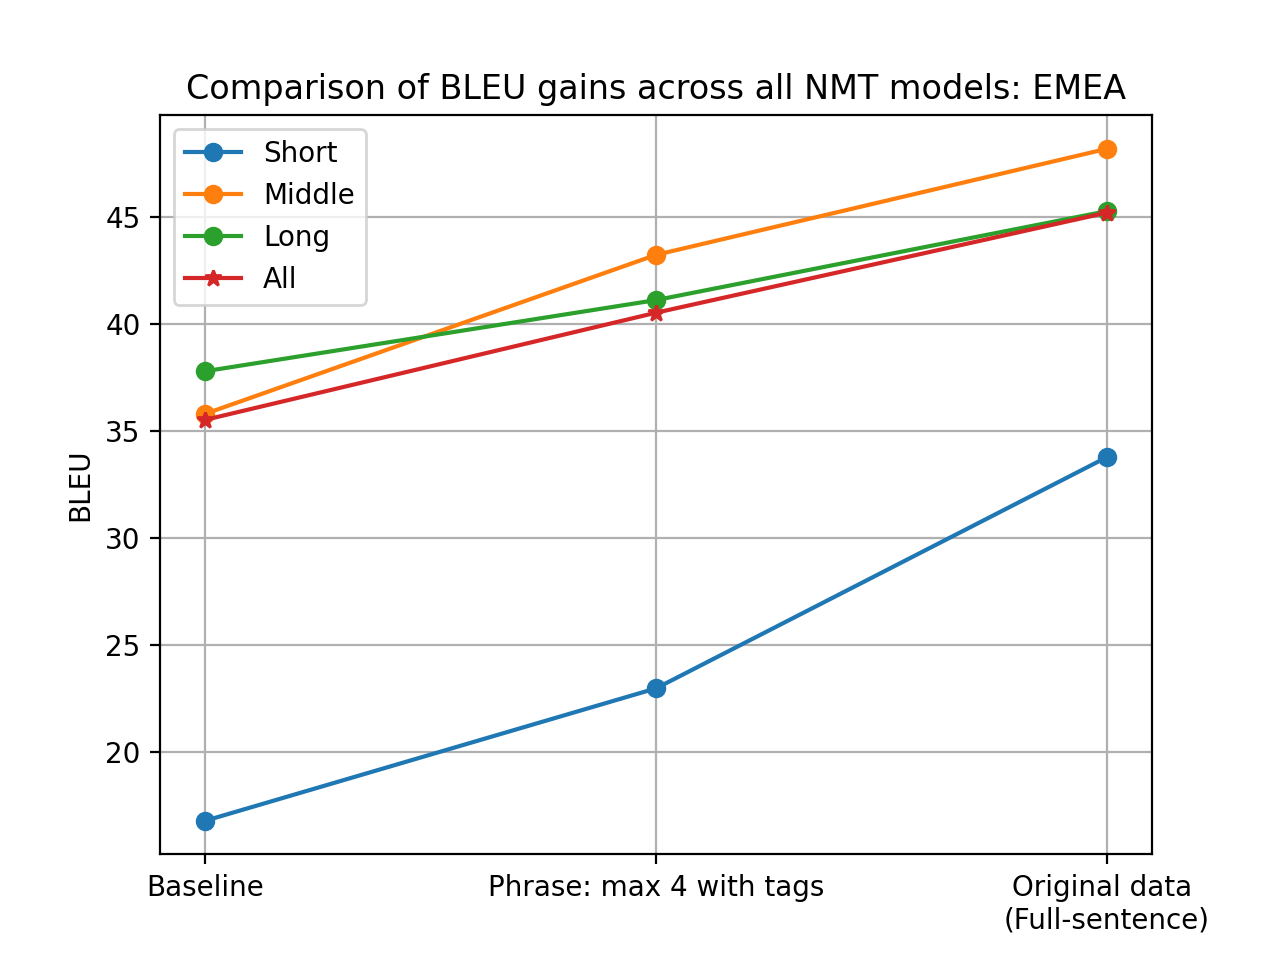
\includegraphics[scale=0.48]{images/EMEA_different_lengths.png}
    \caption{}
    \label{fig:EMEA_different_lengths}
\end{subfigure}
\begin{subfigure}{.48\textwidth}
  \centering
  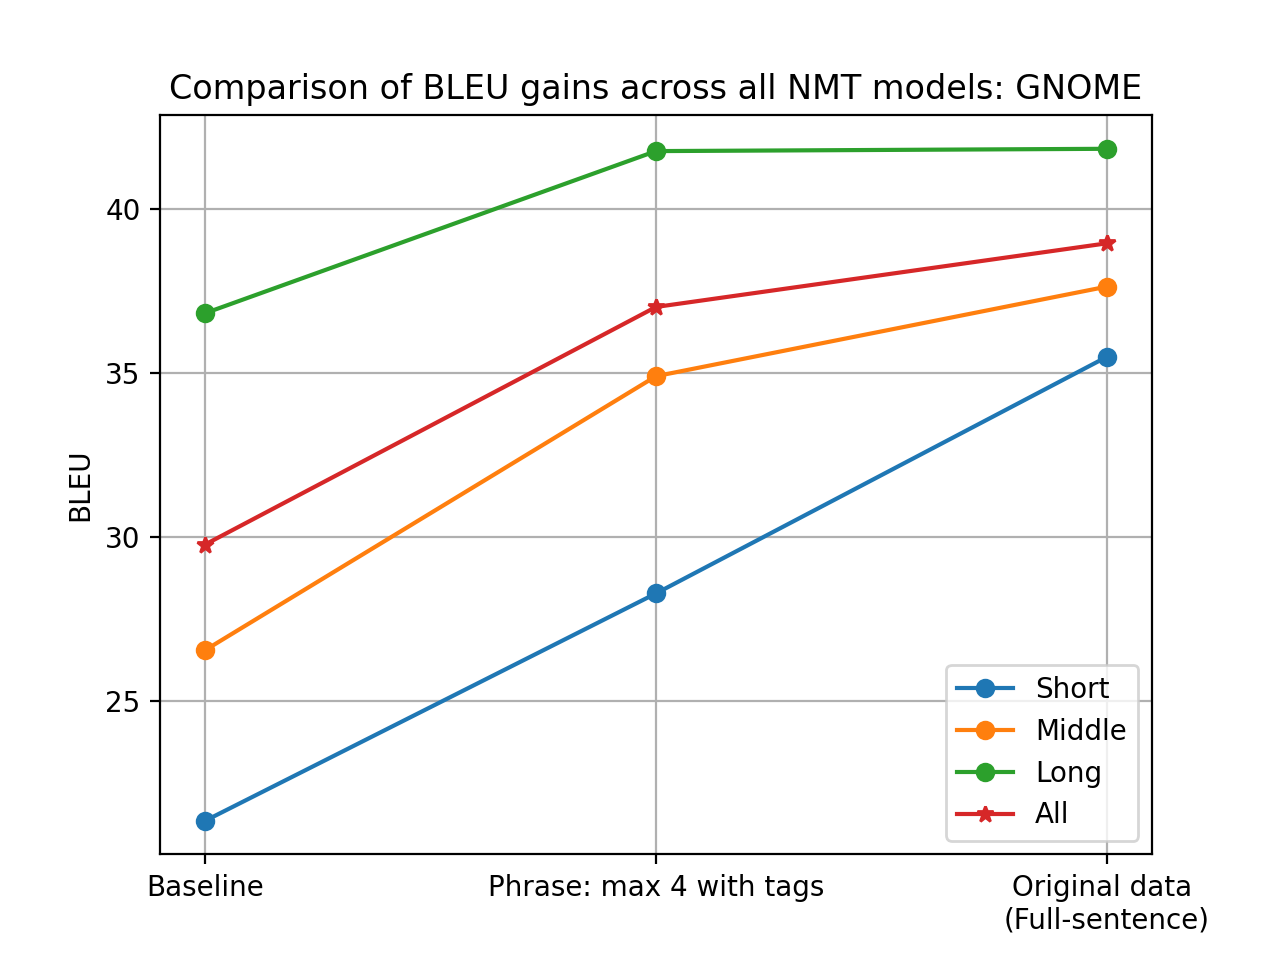
\includegraphics[scale=0.48]{images/GNOME_different_lengths.png}
    \caption{}
    \label{fig:GNOME_different_lengths}
\end{subfigure}
\begin{subfigure}{.48\textwidth}
  \centering
  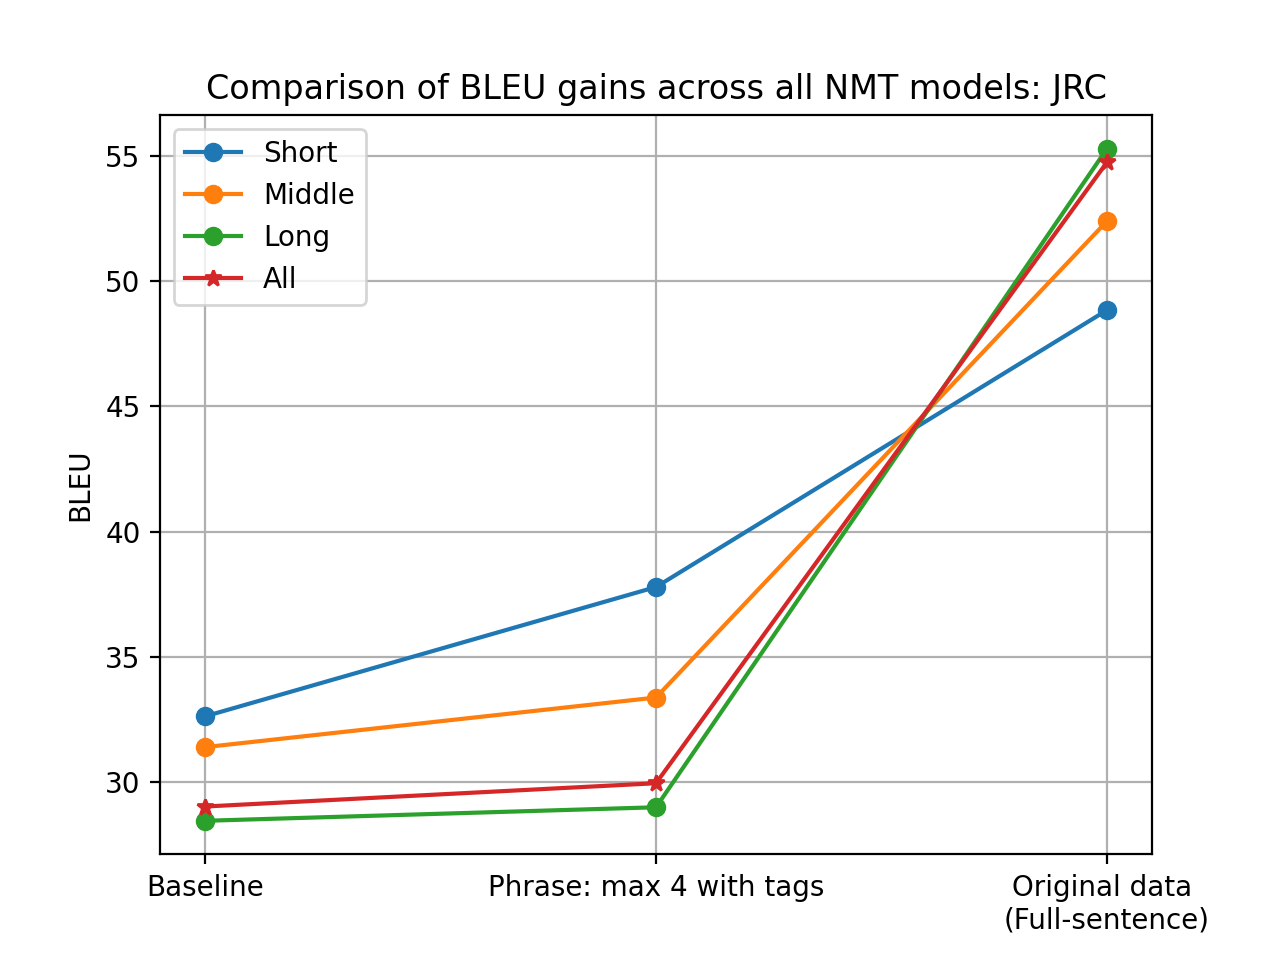
\includegraphics[scale=0.48]{images/JRC_different_lengths.png}
    \caption{}
    \label{fig:JRC_different_lengths}
\end{subfigure}
\caption{Comparison of BLEU gains of all NMT models for various test sets: Baseline, fine-tuning on tagged phrases (max length 4) and fine-tuning on original data(full-sentences). The test set consists of three length groups: short, middle and long (See Table~\ref{tab:lenght_of_sentences} for details)}
\label{fig:different_lengths}
\end{figure}


\subsubsection{Vocabulary differences in domains}

%We expect our pre-trained model to learn the domain specific characteristics while fine-tuning. 
We hypothesise domains which have rich vocabulary to benefit relatively more by fine-tuning on phrases. 
When a domain has a diverse vocabulary, even if the amount of useful information is reduced due to fragmentation of sentences, NMT still can exploit words information through domain adaptation. 

In our experiments, our model uses a Byte Pair Encoding (BPE) to handle new and rare words. Therefore, in order to indicate how many actual vocabularies are in each domain dataset, we count the unique tokens from each training set. In Table \ref{tab:tokens} we report the number of unique tokens in each training set and we included the rates for easy comparison among different sized datasets. The EMEA domain has the largest vocabulary and the JRC domain has the smallest vocabulary. This may explain the results (Table ~\ref{tab:main_results}) where fine-tuning the EMEA dictionary improves the model, but not in other domains.

% \begin{table}[h!]
% \centering
% \begin{tabular}{cc cc cc cc}
% \Xhline{3\arrayrulewidth}
%  &
%   \textbf{} &
%   \multicolumn{2}{c}{\textbf{Original data}} &
%   \multicolumn{2}{c}{\textbf{After applying BPE}} &
%   \multicolumn{2}{c}{\textbf{\begin{tabular}[c]{@{}c@{}}Rate \\ (After BPE / Original)\end{tabular}}} \\ 
%   \cmidrule(lr){3-4}\cmidrule(lr){5-6}\cmidrule(lr){7-8}
% \textbf{}                                            &    & Token  & Vocabulary & Token  & Vocabulary & Token & Vocabulary \\ \hline
% \multicolumn{1}{c}{\multirow{2}{*}{\textbf{EMEA}}}  & De & 198.9K & 7.9K         & 355.4K & 6.2K         & 1.8  & 0.8         \\
% \multicolumn{1}{c}{}                                & En & 209.2K & 6.5K         & 321.7K & 5.5K         & 1.5  & 0.8         \\ \hline
% \multicolumn{1}{c}{\multirow{2}{*}{\textbf{GNOME}}} & De & 179.4K & 10K          & 264.6K & 7.2K         & 1.5  & 0.7         \\
% \multicolumn{1}{c}{}                                & En & 193.6K & 6.8K         & 251.4K & 5.5K         & 1.3  & 0.8         \\ \hline
% \multicolumn{1}{c}{\multirow{2}{*}{\textbf{JRC}}}   & De & 279K & 15.8K          & 395K   & 9.5K         & 1.4  & 0.6         \\
% \multicolumn{1}{c}{}                                & En & 396.2K & 16.8K        & 502.3K & 12.1K        & 1.3  & 0.7         \\ \Xhline{3\arrayrulewidth}
% \end{tabular}
% \caption{General and unique vocabulary for domains.
% The change of dataset after applying BPE}
% \label{tab:tokens}
% \end{table}

\begin{table}[h!]
\centering
\begin{tabular}{cc c c c}
\Xhline{3\arrayrulewidth}
 &
  \textbf{} &
  \multicolumn{1}{c}{\textbf{Before BPE}} &
  \multicolumn{1}{c}{\textbf{After BPE}} &
  \multicolumn{1}{c}{\textbf{\begin{tabular}[c]{@{}c@{}}Rate \\ (After / Before )\end{tabular}}} \\ \hline\hline
  %\cmidrule(lr){3-3}\cmidrule(lr){4-4}\cmidrule(lr){5-5}
% \textbf{}                                            &     & Vocabulary   & Vocabulary  & Vocabulary \\ \hline
\multicolumn{1}{c}{\multirow{2}{*}{\textbf{EMEA}}}  & De  & 7.9K          & 6.2K          & 0.79       \\
\multicolumn{1}{c}{}                                & En  & 6.5K          & 5.5K           & 0.85        \\ \hline
\multicolumn{1}{c}{\multirow{2}{*}{\textbf{GNOME}}} & De  & 10K           & 7.2K          & 0.72         \\
\multicolumn{1}{c}{}                                & En  & 6.8K          & 5.5K           & 0.81         \\ \hline
\multicolumn{1}{c}{\multirow{2}{*}{\textbf{JRC}}}   & De  & 15.8K         & 9.5K          & 0.60         \\
\multicolumn{1}{c}{}                                & En  & 16.8K         & 12.1K          & 0.72         \\ \Xhline{3\arrayrulewidth}
\end{tabular}
\caption{General and unique vocabulary for domains.
The change of dataset after applying BPE}
\label{tab:tokens}
\end{table}


\subsubsection{Similarity between training and test set} %%%%%%%%
% When between training and test sets uplicate or similar sentences  can affect the BLEU score because

A large number of duplicate or similar sentences between the training and test sets may cause the NMT model not to evaluate properly. %and eventually to have a higher BLEU score.
%can affect the BLUE score. 
We try to measure the similarity between training and test sets from every domain and find out which domain has the most similar training and test sets. 
Firstly, we need to define what we mean by the similarity between two datasets. In this thesis, we measure the similarity between two datasets by how many phrases overlap. 
For example, when extracting phrases of the same length from two data sets, the more overlapping phrases, the closer the data sets are. 
The rate of overlapping phrases in the training and test sets for all domains are reported in the Table~\ref{fig:overlapping_phrases}. Since fine-tuning on phrases of the JRC domain has rather low BLEU than other domains, we expected that the similarity rate of the JRC domain is lower than others. 
However, the similarity rates of EMEA and GNOME domains are lower than that of JRC at from 1 to 4 words. Thus, this also cannot provide sufficient explanation why fine-tuning on phrases of the JRC domain gains less than 2 points of BLEU while other domains achieved larger BLEU points. 

\begin{figure}[hb]
    \centering
    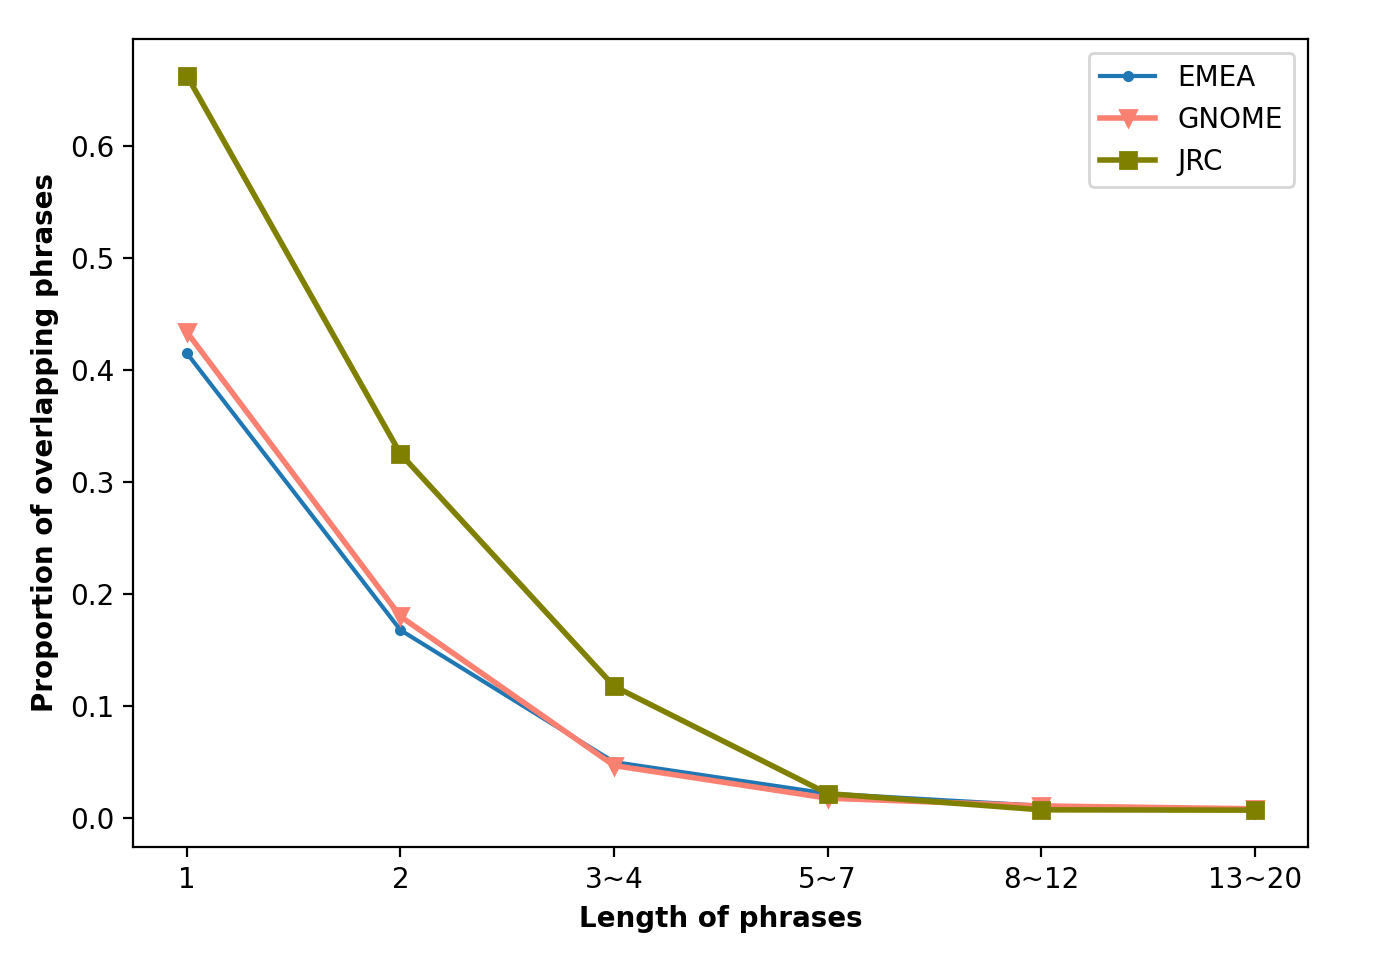
\includegraphics[scale=0.45]{images/overlapping_phrases_all.png}
    \caption{Overlapping phrases in every domain on their corresponding train and test sets.}
    \label{fig:overlapping_phrases}
\end{figure}

\section{Additional Experiments}\label{section:additional_experiments}%%%%%%%%%%%%%%%%%
% Our in-depth analysis on our method of transferring pretrained models, showed that: 1) The method is more advantageous in extremely low-resource scenarios. 2) The method helps to improve the performance over all datasets classes. 3) The method leads to a faster convergence compared to training from scratch. 4) The model’s size does not have an observable effect on the transfer performance. Finally, 5) the pre-training performance on the source task is not a predictor of performance on the target task.
%%%%%%%%%%%%%%%%%%    OTHER RESULTS   %%%%%%%%%%%%%%%
Main results supported that using phrases with the tagging technique for domain adaptation can improve translation quality of NMT models. Based on this, we conducted several additional experiments to boost our approach: 1) Fine-tuning on a mix of out-domain sentences and target domain phrases to mitigate brevity issues.  2) For maximum phrase length 7 data, we set minimum phrase length to prevent very large numbers of segments. The results of it are reported in Table~\ref{tab:other_results_1} and \ref{tab:other_results_2}. 

\begin{table}[h!]
\centering
\begin{tabular}{c|c|ccccccc}
\Xhline{3\arrayrulewidth}
\multirow{3}{*}{} &
  \multirow{3}{*}{\begin{tabular}[c]{@{}c@{}}\textbf{Baseline}\end{tabular}} &
  \multicolumn{7}{c}{\textbf{Fine-Tuning}} \\ \cline{3-9} 
 &
   &
  \multicolumn{3}{c|}{\textbf{Max length 4}} &
  \multicolumn{3}{c|}{\textbf{Max length 7}} &
  \multirow{2}{*}{\begin{tabular}[c]{@{}c@{}}\textbf{Original data}\end{tabular}} \\ \cline{3-8}
 &
   &
  \multicolumn{1}{c|}{\textbf{No tag}} &
  \multicolumn{1}{c|}{\textbf{Tag}} &
  \multicolumn{1}{c|}{\textbf{Mix}} &
  \multicolumn{1}{c|}{\textbf{No tag}} &
  \multicolumn{1}{c|}{\textbf{Tag}} &
  \multicolumn{1}{c|}{\textbf{Mix}} &
   \\ \hline \hline
\textbf{EMEA} &
  \textcolor{gray}{35.5} &
  \multicolumn{1}{c|}{\textcolor{gray}{39.1}} &
  \multicolumn{1}{c|}{\textcolor{gray}{40.5}} &
  \multicolumn{1}{c|}{\cellcolor{red!7}39.6} &
  \multicolumn{1}{c|}{\textcolor{gray}{41.5}} &
  \multicolumn{1}{c|}{\textcolor{gray}{37.2}} &
  \multicolumn{1}{c|}{\cellcolor{red!7}35.4} &
  %\multicolumn{1}{c|}{\cellcolor{blue!7} 41.8} &
  \textcolor{gray}{45.2}
   \\
\textbf{GNOME} &
  \textcolor{gray}{29.8} &
  \multicolumn{1}{c|}{\textcolor{gray}{36.0}} &
  \multicolumn{1}{c|}{\textcolor{gray}{37.0}} &
  \multicolumn{1}{c|}{\cellcolor{red!7}33.7} &
  \multicolumn{1}{c|}{\textcolor{gray}{35.8}} &
  \multicolumn{1}{c|}{\textcolor{gray}{36.8}} &
  \multicolumn{1}{c|}{\cellcolor{red!7}34.8} &
  %\multicolumn{1}{c|}{\cellcolor{blue!7} 32.7} &
  \textcolor{gray}{38.9}
   \\
\textbf{JRC} &
  \textcolor{gray}{29.0} &
  \multicolumn{1}{c|}{\textcolor{gray}{29.4}} &
  \multicolumn{1}{c|}{\textcolor{gray}{30.0}} &
  \multicolumn{1}{c|}{\cellcolor{red!7}29.5} & 
  \multicolumn{1}{c|}{\textcolor{gray}{29.2}} &
  \multicolumn{1}{c|}{\textcolor{gray}{29.7}} &
  \multicolumn{1}{c|}{\cellcolor{red!7}30.5} &
  %\multicolumn{1}{c|}{\cellcolor{blue!7} 30.2} &
  \textcolor{gray}{54.7}
   \\ \Xhline{3\arrayrulewidth}
\end{tabular}
\caption{The BLEU scores of the additional experimental results are compared with the BLUE scores of the main results. The fine-tuning results for mix of out-domain full sentences and in-domain phrases are reported.}
\label{tab:other_results_1}
\end{table}
\subsection{Mixed data : in-domain phrases and out-domain sentences}

Besides the tagging technique, we also consider fine-tuning on a mix of in-domain phrases and out-domain full sentences to avoid the shorter output bias. For the out-domain sentences, because the baseline model was trained on previous years WMT newstest sets, including newstest2012, newstest2013, newstest2015 and newstest2017, we reserve 5K sentences from them. The out-domain sentences are mixed with the tagged phrases to generate a mixed dataset and we fine-tune the NMT model with this.

The results are reported in Table~\ref{tab:other_results_1}. Contrary to what we expected, fine-tuning on mix datasets cannot improve the BLEU scores over the tagging technique except the JRC domain with max length 7, and decrease BLEU. Furthermore, in most cases, BLEU was decreased or only similar compared to that fine-tuning on pure phrases.


\subsection{Setting minimum length for maximum length 7 phrases}
%If an element is duplicated in the training data, it is effectively the same as having its 'weight' doubled. That element becomes twice as important when the classifier is fitting your data, and the classifier becomes biased towards correctly classifying that particular scenario over others.

We hypothesised that the long phrases may contain more information than short phrases but we could not observe that longer phrases are more informative than shorter ones for fine-tuning. 
However, as we mentioned in Section~\ref{section:effect_phrase_length}, we suspect this is due to the interference of the bigger number of duplicate and overlapping phrases in the phrases of the bigger number of maximum length. After extracting phrases from the original full sentences, due to the way of extraction process, increasing the maximum length leads to a much larger number of extracted phrases that are redundant and overlapping. In fact, when extracting phrase pairs with a maximum length of 7, the lengths of 1 to 7 phrases are included, and more phrases of each length are extracted than when the maximum length is 4. 
To reduce the effect of this overlapping phrase, we experiment with a minimum phrase length when we use a maximum length of 7 phrases for fine-tuning. For fine-tuning, we remove phrases that are shorter than 5 from the extracted phrases with a maximum length of 7. Furthermore, we conduct this experiment with and without tags. 

\begin{table}[b!]
\centering
\begin{tabular}{c|c|ccccccc}
\Xhline{3\arrayrulewidth}
\multirow{3}{*}{} &
  \multirow{3}{*}{\begin{tabular}[c]{@{}c@{}}\textbf{Baseline}\end{tabular}} &
  \multicolumn{6}{c}{\textbf{Fine-Tuning}} \\ \cline{3-9} 
 &
   &
  \multicolumn{2}{c|}{\textbf{Max length 4}} &
  \multicolumn{4}{c|}{\textbf{Max length 7}} &
  \multirow{2}{*}{\begin{tabular}[c]{@{}c@{}}\textbf{Original} \\ \textbf{data}\end{tabular}} \\ \cline{3-8}
 &
   &
  \multicolumn{1}{c|}{\textbf{No tag}} &
  \multicolumn{1}{c|}{\textbf{Tag}} &
  \multicolumn{1}{c|}{\textbf{No tag}} &
  \multicolumn{1}{c|}{\textbf{Min 5 no tag}} &
  \multicolumn{1}{c|}{\textbf{\small{Tag}}} &
  \multicolumn{1}{c|}{\textbf{\small{Min 5 tag}}} &
   \\ \hline \hline
\textbf{EMEA} &
  \textcolor{gray}{35.5} &
  \multicolumn{1}{c|}{\textcolor{gray}{39.1}} &
  \multicolumn{1}{c|}{\textcolor{gray}{40.5}} &
  \multicolumn{1}{c|}{\textcolor{gray}{41.5}} &
  \multicolumn{1}{c|}{\cellcolor{blue!7} 40.2} &
  \multicolumn{1}{c|}{\textcolor{gray}{37.2}} &
  \multicolumn{1}{c|}{\cellcolor{blue!7} 41.8} &
  \textcolor{gray}{45.2}
   \\
\textbf{GNOME} &
  \textcolor{gray}{29.8} &
  \multicolumn{1}{c|}{\textcolor{gray}{36.0}} &
  \multicolumn{1}{c|}{\textcolor{gray}{37.0}} &
  \multicolumn{1}{c|}{\textcolor{gray}{35.8}} &
  \multicolumn{1}{c|}{\cellcolor{blue!7} 35.8} &
  \multicolumn{1}{c|}{\textcolor{gray}{36.8}} &
  \multicolumn{1}{c|}{\cellcolor{blue!7} 32.7} &
  \textcolor{gray}{38.9}
   \\
\textbf{JRC} &
  \textcolor{gray}{29.0} &
  \multicolumn{1}{c|}{\textcolor{gray}{29.4}} &
  \multicolumn{1}{c|}{\textcolor{gray}{30.0}} &
  \multicolumn{1}{c|}{\textcolor{gray}{29.2}} &
  \multicolumn{1}{c|}{\cellcolor{blue!7} 30.2} &
  \multicolumn{1}{c|}{\textcolor{gray}{29.7}} &
  \multicolumn{1}{c|}{\cellcolor{blue!7} 30.2} &
  \textcolor{gray}{54.7}
   \\ \Xhline{3\arrayrulewidth}
\end{tabular}
\caption{The BLEU scores of the additional experimental results are compared with the BLUE scores of the main results. The fine-tuning results for phrases that consist of 5 up to 7 words are reported.}
\label{tab:other_results_2}
\end{table}

The results are reported in Table~\ref{tab:other_results_2}. In the EMEA and JRC domains, fine-tuning on phrase length 5$\sim$7 has the higher BLEU scores than on phrases length 4. On the GNOME domain, the BLUE score of fine-tuning on phrases length 5$\sim$7 stays compared to maximum length 7. On the other hand, when using the tagging technique, the effect of reducing redundant phrases is +1.6 BLEU on EMEA, -3.1 BLEU on GNOME and maintained on JRC. To sum up, setting the minimum length of phrases does not confer a positive effect on the BLUE score.




\subsection{Qualitative analysis: Translation examples} %%%%%%%%%%

To give an overview of what the generated translations look like, we provide some examples of outputs and reference as a qualitative analysis. We want to utilise this to find interesting patterns that might have been missed when the experimental results are analysed only through statistical analysis.

Table~\ref{tab:EMEA_sample} shows reference and samples of the domain EMEA. We often observe in the output from phrase-adapted models that the first word of the sentences are missing or no capital letters for the first words. %In the example, it shows that in green that except for fine-tuning on the tagged max 4 phrases. 
Different vocabularies are used for generating output from the NMT models. In this example, ''threat'' in the reference sentence is translated into ''danger'' in the baseline ''risk'' for all other NMT models. In addition, the translation lengths of the phrase-adapted models are slightly shorter than non-adapted and sentence-adapted models. Another examples of translations in the EMEA domain are reported in Table~\ref{tab:EMEA_sample_1} and again we observe the most phrase-adapted models use more technical word (paediatric) than baseline and sentence-adapted model (children).

\begin{table}[htb]
\centering
\begin{tabular}{P{0.17\linewidth}  p{0.8\linewidth}}
\Xhline{3\arrayrulewidth}
                       & \multicolumn{1}{c}{\textbf{Output}}\\ \hline
\textbf{Source}        & Injektion alle 8-24 Stunden (6-12 Stunden bei Patienten unter 6 Jahren) wiederholen, bis die Gefahr für den Patienten vorüber ist. \\ \hline
\textbf{Reference}     & Repeat injections every 8 to 24 hours (6 to 12 hours for patients under the age of 6) until \textcolor{blue}{threat} is resolved.  \\
\textbf{Baseline}      & Repeat the injection every 8-24 hours (6-12 hours in patients under 6 years of age) until the \textcolor{blue}{danger} to the patient is over.       \\
\textbf{No tag, max 4} & \textcolor{violet}{injection} every 8-24 hours (6-12 hours in patients under 6 years of age) until the \textcolor{blue}{risk} to the patient is over.  \\
\textbf{Tagged max 4}  & Repeat the injection every 8-24 hours (6-12 hours in patients under 6 years of age) until the \textcolor{blue}{risk} to the patient is over.         \\
\textbf{No tag, max 7} & \textcolor{violet}{injection} every 8-24 hours (6-12 hours for patients under 6 years of age) until the \textcolor{blue}{risk} to the patient is over. \\
\textbf{Tagged max 7}  & \textcolor{violet}{injection} every 8-24 hours (6-12 hours for patients less than 6 years) until the \textcolor{blue}{risk} to the patient is over.    \\
\textbf{Original data} & Repeat the injection every 8-24 hours (6-12 hours in patients under 6 years of age) until the \textcolor{blue}{risk} to the patient is over.         \\ \Xhline{3\arrayrulewidth}
\end{tabular}
\caption{Translation samples: EMEA}
\label{tab:EMEA_sample}
\end{table}

\begin{table}[H]
\centering
\begin{tabular}{P{0.17\linewidth}  p{0.8\linewidth}}
\Xhline{3\arrayrulewidth}
                       & \multicolumn{1}{c}{\textbf{Output}}\\ \hline
\textbf{Source}        & Diese Wirkungen sind bei Kindern, älteren Patienten oder im Falle einer Überdosierung wahrscheinlicher \\ \hline
\textbf{Reference}     & These effects may be more likely to occur in \textcolor{blue}{children}, elderly patients, or in cases of overdose \\
\textbf{Baseline}      & These effects are more likely in \textcolor{blue}{children}, elderly patients or in the event of an overdose \\
\textbf{No tag, max 4} & These effects are more likely in \textcolor{blue}{paediatric}, elderly patients, or in case of overdose  \\
\textbf{Tagged max 4}  & These effects are more likely in \textcolor{blue}{paediatric}, elderly patients or in case of overdose         \\
\textbf{No tag, max 7} & These effects are more likely in \textcolor{blue}{paediatric}, elderly patients or in the case of overdose \\
\textbf{Tagged max 7}  & These effects are more likely in \textcolor{blue}{children}, the elderly or in the case of overdose    \\
\textbf{Original data} & These effects are more likely in \textcolor{blue}{children}, elderly patients or in the event of an overdose \\ \Xhline{3\arrayrulewidth}
\end{tabular}
\caption{Translation samples: EMEA}
\label{tab:EMEA_sample_1}
\end{table}

\begin{table}[h!]
\centering
\begin{tabular}{P{0.17\linewidth}  p{0.8\linewidth}}
\Xhline{3\arrayrulewidth}
                      & \multicolumn{1}{c}{\textbf{Output}} \\ \hline
\textbf{Source}        &  Spiele könnten nur teilweise übersetzt sein, so dass es schwieriger ist, diese zu spielen. \\ \hline
\textbf{Reference}     &  You may be exposed to partially \textcolor{blue}{translated} games making it more difficult to play. \\
\textbf{Baseline}      &  Games may only be partially \textcolor{blue}{translated}, so it is more difficult to play them.\\
\textbf{No tag, max 4} &  \textcolor{violet}{games} might only be partially \textcolor{blue}{translated}, so it is more difficult to play them. \\
\textbf{Tagged max 4}  &  Games might only be partially \textcolor{blue}{compiled}, so it is more difficult to play them. \\
\textbf{No tag, max 7} &  \textcolor{violet}{games} might only be partially \textcolor{blue}{compiled}, so it is more difficult to play them. \\
\textbf{Tagged max 7}  &  Games might only be partially \textcolor{blue}{compiled}, so it is more difficult to play them. \\
\textbf{Original data} &  Games might be only partially \textcolor{blue}{translated}, making them more difficult to play. \\ \Xhline{3\arrayrulewidth}
\end{tabular}
\caption{Translation samples: GNOME}
\label{tab:GNOME_sample}
\end{table}

In Table~\ref{tab:GNOME_sample} we report translation samples of the GNOME domain. As mentioned earlier, this sample also has the lowercase error of the first word in the translation of the phrase-adapted models without tags. Some of the translation of the models fine-tuned on phrases contain domain-specific words compared to other models. This pattern can also be seen in the sample, where the word ''translated'' is translated into a software-related word 'compiled' (GNOME is software domain).

% \begin{table}[ht!]
% \centering
% \begin{tabular}{P{0.17\linewidth}  p{0.8\linewidth}}
% \Xhline{3\arrayrulewidth}
%                       & \multicolumn{1}{c}{\textbf{Output}} \\ \hline
% \textbf{Source}        & gbrainy ist ein unterhaltsames Spiel, um das Gehirn zu trainieren. Es enthält: \\ \hline
% \textbf{Reference}     & gbrainy is a brain teaser game and trainer to have fun and to keep your brain trained. It includes:\\
% \textbf{Baseline}      & gbrainy is an entertaining game to train the brain. It contains: \\
% \textbf{No tag, max 4} & gbrainy is an entertaining game to train the brain. It contains: \\
% \textbf{Tagged max 4}  & gbrainy is a fun game to train the brain. It contains: \\
% \textbf{No tag, max 7} & gbrainy is a fun game to train the brain. It contains: \\
% \textbf{Tagged max 7}  & gbrainy is a fun game to train the brain. It contains:\\
% \textbf{Original data} & gbrainy is an entertaining game to train the brain. It contains:\\ \Xhline{3\arrayrulewidth}
% \end{tabular}
% \caption{GNOME}
% \label{tab:sample}
% \end{table}

\subsection{The JRC domain} 

\begin{table}[h!]
\centering
\begin{tabular}{cccc}
\Xhline{3\arrayrulewidth}
\multicolumn{2}{c}{}        & \textbf{Train}                        & \textbf{Test}                                 \\ \hline
\multirow{2}{*}{\textbf{EMEA}}  & De & 20.9   & 19.8  \\
                       & En & 21.9 & 21.8           \\ \hline
\multirow{2}{*}{\textbf{GNOME}} & De & 18.9   & 15.3         \\
                       & En & 20.4  & 15.8        \\ \hline
\multirow{2}{*}{\textbf{JRC}}   & De & 28.9  & 27.7  \\
                       & En & 40.6  & 41.9  \\\Xhline{3\arrayrulewidth}
\end{tabular}
\caption{The average length of sentences from each dataset}
\label{Tab:mean_sentences}
\end{table}

% Analyzing Uncertainty in Neural Machine Translation \\
%     "A lesser-known example are target sentences which are entirely in the source language, or which are primarily copies of the corresponding source." : This is exactly the case of JRC that has lots of copies. 
We conducted several analyses to answer why the BLEU gains of fine-tuning for JRC phrases is insignificant, but we could not find a good explanation. However, we found that the average length of English sentences of JRC datasets considerably longer than German, more than 10 words, as Table \ref{Tab:mean_sentences} shows. Therefore, we analyse the reference and translation results of JRC, we detect a noise in the JRC dataset that some source sentences are copied in the target side.
%The JRC domain is composed of longer sentences than other domains and especially, English sentences are longer than German sentences, more than 10 words long. 
%Furthermore, why does JRC's result of phrases have lower performance than original dataset, and for the other 2 domain datasets phrases works better than their original dataset?
%While we analyse translation results of JRC, we detect a noise in JRC dataset that some source sentences are copied in target side. 
In other words, where the source sentence is \textbf{S} and its translation is \textbf{T}, the noised target reference consist of \textbf{S} and \textbf{T} together. An example of this noise is reported in Table~\ref{tab:sample_JRC} where the reference has the copy of source sentence. We suspect that the phrase-adapted model could not learn the noise, while fine-tuning on original data could. Furthermore, when we extract the phrases with this noise, the quality of phrases may drop. 

\begin{table}[H]
\centering
\begin{tabular}{P{0.17\linewidth}  p{0.8\linewidth}}
\Xhline{3\arrayrulewidth}

                     & \multicolumn{1}{c}{\textbf{Output}} \\ \hline
\textbf{Source}        & Der Missionsleiter der EUMM wird vom Rat der Europäischen Union ernannt.

 \\ \hline
\textbf{Reference}     &  \textcolor{red}{Der Missionsleiter der EUMM wird vom Rat der Europäischen Union ernannt.} The Head of Mission of the EUMM shall be appointed by the Council of the European Union.\\
\textbf{Baseline}      & The Head of Mission of the EUMM shall be appointed by the Council of the European Union.
 \\
\textbf{No tag, max 4} & The Head of Mission of the EUMM shall be appointed by the Council of the European Union.
\\
\textbf{Tagged max 4}  & The Head of Mission of the EUMM shall be appointed by the Council of the European Union.
\\
\textbf{No tag, max 7} &  The Head of Mission of the EUMM shall be appointed by the Council of the European Union.
 \\
\textbf{Tagged max 7}  & The Head of Mission of the EUMM shall be appointed by the Council of the European Union.
 \\
\textbf{Original data} &  \textcolor{red}{Der Missionsleiter der EUMM wird vom Rat der Europäischen Union ernannt.} The Head of Mission of the EUMM shall be appointed by the Council of the European Union. \\ \Xhline{3\arrayrulewidth}
\end{tabular}
\caption{Translation sample of JRC. This sample shows the noise that the target reference consists of copy of source sentence and its translation. Fine-tuning on whole original sentences can learn this noise but for on phrases cannot.}
\label{tab:sample_JRC}
\end{table}

We would like to investigate how this noise affects the translation quality in fine-tuning on the JRC domain. 
We remove this noise from the JRC datasets to create new JRC dataset and also extract new phrases from the new training set. Then, we fine-tune the NMT model on the new JRC datasets. The results is reported in Table~\ref{tab:new_JRC}. The baseline improves +7.6 BLEU but fine-tuning on full sentences deteriorates -16 BLEU. In other words, the potential gain of domain adaptation significantly decreases. The BLEU score of the phrase-adapted model (with tags, max 4) increases +0.7 BLEU and close to the ceiling. This shows that removing the noise affect significantly the BLEU scores of the JRC domain. 



\begin{table}[H]
\centering
\begin{tabular}{c|c|c|c}
\Xhline{3\arrayrulewidth}
\multirow{2}{*}{} &
  \multirow{2}{*}{\begin{tabular}[c]{@{}c@{}}\textbf{Baseline}\\ (No fine-tuning)\end{tabular}} &
  \multicolumn{2}{c}{\textbf{Fine-tuning}} \\ \cline{3-4} 
 &
   &
  \textbf{Tagged max 4 phrase} &
  \begin{tabular}[c]{@{}c@{}} \textbf{Original data}\\ (Full sentences)\end{tabular} \\ \hline \hline
\textbf{New JRC}      & 37.6 & 38.3 & 38.7 \\ \hline
\textbf{Original JRC} &  29.0 &   30.0 & 54.7 \\ \Xhline{3\arrayrulewidth}
\end{tabular}
\caption{BLEU scores of the baseline, the phrase-adapted model (with tag, maximum length 4) , and the sentence-adapted model fine-tuned on the old JRC and new JRC datasets.}
\label{tab:new_JRC}
\end{table}